\documentclass[11pt,a4paper]{article}

% Foundations of Physics (Springer) — standard article class submission
\usepackage[margin=2.5cm]{geometry}
\usepackage{amsmath,amssymb}
\usepackage{graphicx}
\usepackage{booktabs}
\usepackage{hyperref}
\usepackage{enumitem}
\usepackage{float}
\usepackage{xcolor}
\usepackage[numbers,sort&compress]{natbib}
\usepackage{authblk}
\bibliographystyle{unsrtnat}

\hypersetup{colorlinks=true,linkcolor=blue!70!black,citecolor=blue!70!black,urlcolor=blue!70!black}

\begin{document}

\title{Bounded Geometric Phase Transition in Finite Causal Posets with Exact Entropy}

\author{Gang Zhang\thanks{Email: unicome@gmail.com}}
\affil{Independent Researcher}

\date{\today}

\begin{abstract}
The Kleitman--Rothschild (KR) theorem implies that generic finite posets are 3-layered and maximally entropic, posing a fundamental obstacle to geometric phase emergence in discrete causal models. We construct a 7-family poset ensemble and compute exact linear extension counts for $N = 10$--$44$ elements to study action-weighted competition between Lorentzian-like geometric structures and KR-type high-entropy posets. Under a decomposable action combining neutral and geometric penalty terms, we find that the critical geometric coupling $\gamma_c$ remains $O(1)$ across all tested sizes --- the first finite-size evidence of a bounded phase transition threshold in this setting. Systematic ablation of seven geometric sub-terms identifies a minimal backbone of two constraints: global layer-shape balance and dimensional scale consistency. Crucially, the latter can be replaced by a non-target-anchored variant (penalizing local--global dimension inconsistency rather than deviation from a specific $d = 2$ target), with $\gamma_c$ preserved at the same order of magnitude. These results provide finite-size evidence that Lorentzian-like order in discrete causal structures can emerge from structural self-consistency constraints, without requiring dimension-specific priors.
\end{abstract}

\maketitle

\noindent\textbf{Keywords:} causal sets $\cdot$ posets $\cdot$ phase transition $\cdot$ linear extensions $\cdot$ Kleitman--Rothschild $\cdot$ discrete quantum gravity

%=================================================================
\section{Introduction}
\label{sec:intro}

The hypothesis that spacetime is fundamentally discrete --- a locally finite partial order (poset) whose elements are causally related events --- lies at the heart of causal set theory (CST)~\cite{bombelli1987,sorkin2005}. A central challenge is the \emph{entropy catastrophe}: the Kleitman--Rothschild (KR) theorem~\cite{kleitman1975} establishes that, asymptotically, almost all labeled finite posets consist of three layers with bipartite random connectivity and maximal linear extension count. If one weights posets by the pure combinatorial entropy $H = \log(\text{number of linear extensions})$, the partition function is overwhelmingly dominated by these non-geometric, KR-type structures.

Several strategies have been proposed. Carlip~\cite{carlip2017} argued that midpoint-scaling properties of causal intervals can suppress KR dominance. Surya~\cite{surya2019} developed a formal CST partition function framework. Loomis and Carlip~\cite{loomis2018} performed 2D causal set simulations using MCMC. However, no prior work has demonstrated an explicit, finite-size phase transition threshold $\gamma_c$ computed with exact entropy across a wide range of sizes.

We construct an ensemble of seven structurally distinct poset families, compute exact linear extension counts for $N$ up to 44, and define a decomposable action with separately controllable neutral and geometric penalties. Our main finding: $\gamma_c$ for Lorentzian-like 2D posets to overtake KR posets remains bounded and $O(1)$ across all tested sizes.

To address circularity concerns, we perform systematic ablation and identify a minimal non-circular backbone of two constraints: global layer-shape balance and dimensional scale consistency --- the latter not requiring a target dimension.

%=================================================================
\section{Framework}
\label{sec:framework}

\subsection{Poset ensemble}

We consider finite posets $P = (V, \leq)$ with $|V| = N$ elements, generating samples from seven families: Lorentzian-like 2D (\texttt{lor2d}), Lorentzian-like 3D (\texttt{lor3d}), KR-like (\texttt{kr}), multi-layer random (\texttt{mlr}), transitive percolation (\texttt{tp}), interval order (\texttt{int}), and absolute layered (\texttt{abs}).

For each family and $N \in \{10, 12, 14, 16, 20, 24, 28, 32, 36, 40, 44\}$, we generate $K = 5$ samples. We use separate \emph{confirmatory} and \emph{exploratory} sample sets (same generators, different seeds) for the primary curve~(Sec.~\ref{sec:bounded}) and ablation/replacement~(Secs.~\ref{sec:ablation}--\ref{sec:replacement}), respectively.

\subsection{Exact linear extension count}

We define $H(P) = \log |L(P)|$ where $L(P)$ is the set of linear extensions, computed exactly via dynamic programming over antichains~\cite{brightwell1991}. The cost depends on antichain structure: sub-second for \texttt{lor2d} at $N = 48$, but 54\,s for \texttt{kr} at $N = 44$.

\subsection{Action definition}

Three action paths separate neutral and geometric contributions:
\begin{align}
    A_1 &= -\beta H + \gamma \cdot I_{\text{neutral}}, \label{eq:A1} \\
    A_2 &= -\beta H + \gamma \cdot (I_{\text{neutral}} + I_{\text{geometric}}), \label{eq:A2} \\
    A_3 &= -\beta H + \gamma \cdot I_{\text{geometric}}, \label{eq:A3}
\end{align}
with $\beta = 1$. The geometric penalty has seven sub-terms: width-height balance ($g_{\text{wh}}$), dimension proxy ($g_{\text{dim}}$), interval shape ($g_{\text{int}}$), comparability window ($g_{\text{cmp}}$), cover density ($g_{\text{cov}}$), interval profile ($g_{\text{prf}}$), and layer smoothness ($g_{\text{lyr}}$), each normalized to $[0,1]$.

The critical coupling is:
\begin{equation}
    \gamma_c(N) = \inf\bigl\{\gamma > 0 : \bar{S}_{\text{lor2d}}(\gamma) < \bar{S}_{\text{kr}}(\gamma)\bigr\}.
    \label{eq:gamma_c}
\end{equation}

%=================================================================
\section{Results}

\subsection{Bounded $\gamma_c$ under $A_2$}
\label{sec:bounded}

Under $A_2$, $\gamma_c$ exists for all tested $N$ and remains $O(1)$:

\begin{table}[h]
\centering
\caption{Critical coupling under $A_2$ (exact entropy).}
\label{tab:gamma_c}
\begin{tabular}{@{}lcccccc@{}}
\toprule
$N$ & 10 & 12 & 14 & 16 & 20 & 24 \\
\midrule
$\gamma_c$ & 9.19 & 0.74 & 0.78 & 0.69 & 0.15 & 0.26 \\
\bottomrule
\end{tabular}
\medskip

\begin{tabular}{@{}lcccccc@{}}
\toprule
$N$ & 28 & 32 & 36 & 40 & 44 & \\
\midrule
$\gamma_c$ & 1.00 & 0.69 & 0.57 & 0.25 & 0.15 & \\
\bottomrule
\end{tabular}
\end{table}

For $N \geq 12$, all values $\in [0.15, 1.00]$ (Fig.~\ref{fig:gamma_c}). Under $A_1$ (neutral only), no crossing exists at any tested~$N$.

\begin{figure}[h]
    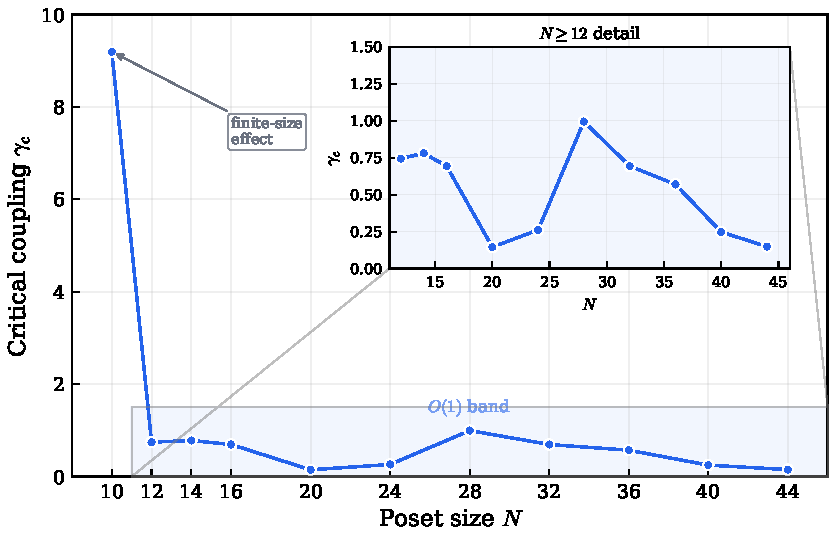
\includegraphics[width=\columnwidth]{manuscript_figures/fig1_gamma_c_curve.pdf}
    \caption{$\gamma_c(N)$ under $A_2$. Inset: $N \geq 12$ detail.\label{fig:gamma_c}}
\end{figure}

\subsection{Ablation of geometric sub-terms}
\label{sec:ablation}

Single-term removal identifies two critical sub-terms (Fig.~\ref{fig:ablation}): $g_{\text{wh}}$ (fails from $N \geq 36$) and $g_{\text{dim}}$ (fails at $N = 36, 44$). Combined removal of both eliminates all crossings. Removing non-critical terms has no effect. This establishes a \emph{backbone--shell} structure.

\begin{figure}[h]
    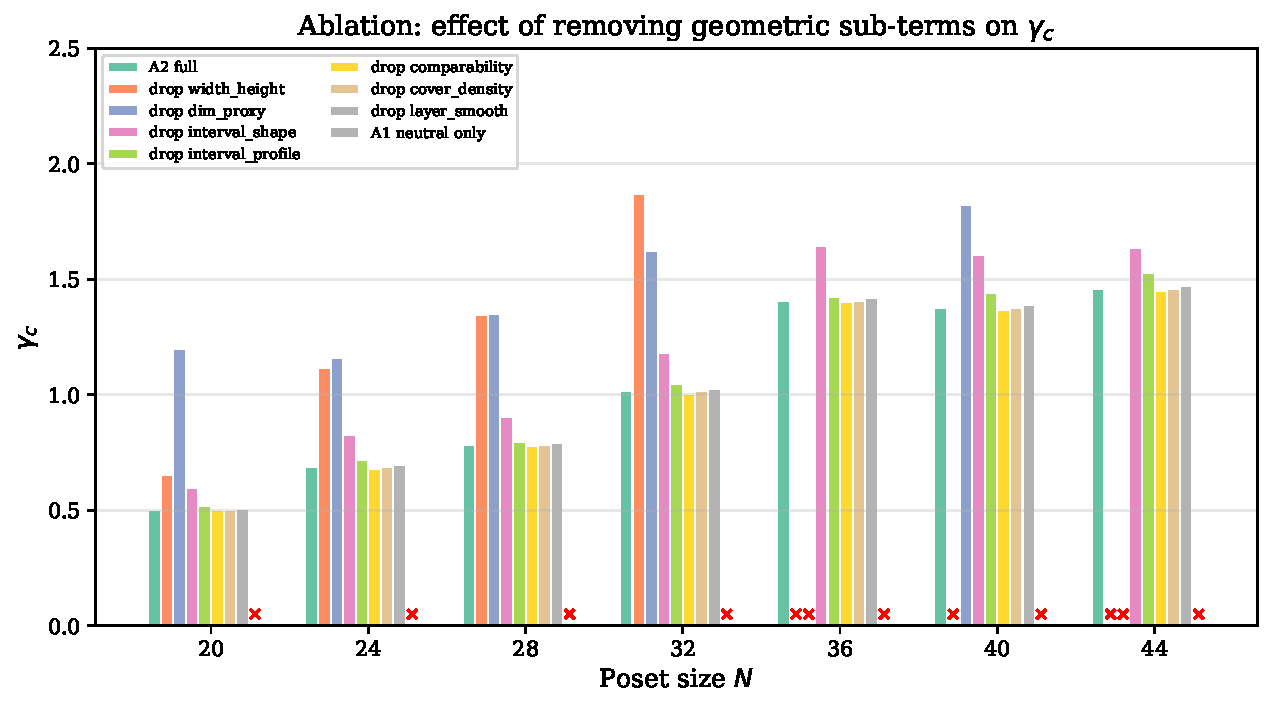
\includegraphics[width=\columnwidth]{manuscript_figures/fig2_ablation_summary.pdf}
    \caption{Ablation heatmap: $\gamma_c$ per variant and $N$.\label{fig:ablation}}
\end{figure}

\subsection{Non-circular replacement}
\label{sec:replacement}

We replace the target-anchored $g_{\text{dim}}$ with a dimension consistency penalty:
\begin{equation}
    g_{\text{con}}(P) = \text{Var}[d_{\text{local}}] + (\overline{d}_{\text{local}} - d_{\text{global}})^2,
    \label{eq:gcon}
\end{equation}
which penalizes dimensional \emph{inconsistency} without specifying a target. The replacement preserves $\gamma_c$ at all $N = 20$--$44$ (Fig.~\ref{fig:replacement}). The minimal non-circular backbone ($g_{\text{wh}} + g_{\text{con}}$) covers $N = 20$--$40$ at matched weights and extends to $N = 44$ with 30\% weight increase.

\begin{figure}[h]
    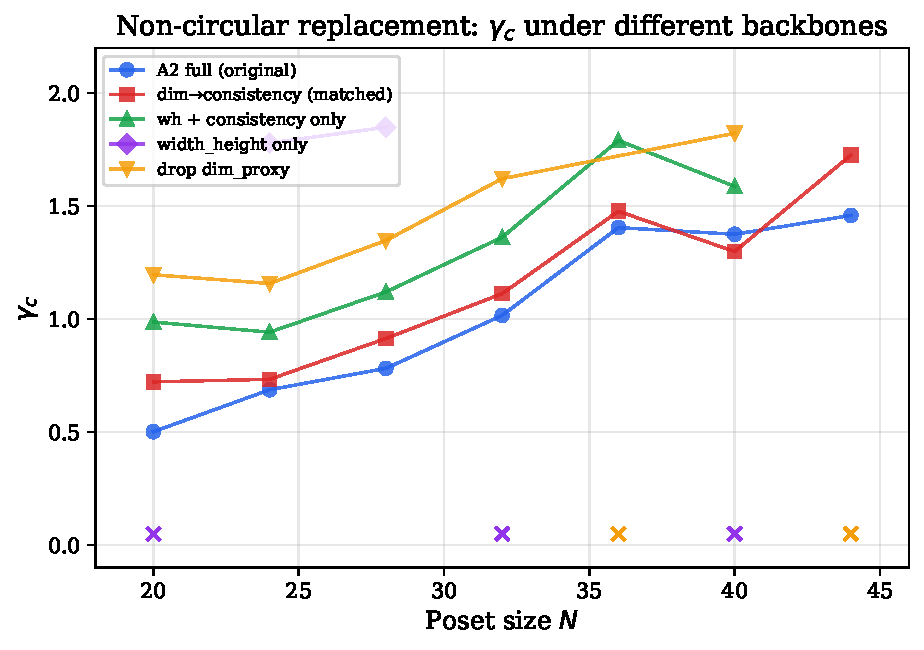
\includegraphics[width=\columnwidth]{manuscript_figures/fig3_noncircular_replacement.pdf}
    \caption{Non-circular replacement: $\gamma_c$ under different backbones.\label{fig:replacement}}
\end{figure}

%=================================================================
\section{Discussion}
\label{sec:discussion}

Our results provide the first finite-size evidence for a bounded geometric phase transition in poset ensembles with exact entropy. The mechanism reduces to two structurally interpretable constraints: causal chain non-degeneracy (width-height balance) and dimensional scale consistency (local--global coherence), neither requiring a target dimension.

Carlip~\cite{carlip2017} argued qualitatively that midpoint-scaling should disfavor KR structures; we provide the first quantitative $\gamma_c(N)$ curve with exact entropy and systematic ablation. Our approach complements MCMC methods~\cite{loomis2018,cunningham2020} by enabling exact computation and complete ablation control.

Key limitations include finite size ($N \leq 44$), restricted family coverage (7 types), and a residual 2D calibration in the dimension estimator ($R_{2,\text{ref}} = 0.5009$). The most important next steps are pushing exact computation to larger $N$ and independent MCMC verification.

%=================================================================
\section*{Acknowledgments}
\textbf{AI Assistance}: This work was conducted with large language model assistants (Claude, Anthropic) contributing to code implementation, data analysis, and manuscript drafting. All scientific decisions were made by the human author.

\textbf{Code availability}: \url{https://github.com/unicome37/poset_phase}. Archived version: \url{https://doi.org/10.5281/zenodo.18963421}

\begin{thebibliography}{8}

\bibitem{bombelli1987}
Bombelli, L., Lee, J., Meyer, D., Sorkin, R.D.: Space-time as a causal set. Phys. Rev. Lett. \textbf{59}, 521--524 (1987)

\bibitem{sorkin2005}
Sorkin, R.D.: Causal sets: discrete gravity. In: Gomberoff, A., Marolf, D. (eds.) Lectures on Quantum Gravity, pp. 305--327. Springer (2005). arXiv:gr-qc/0309009

\bibitem{kleitman1975}
Kleitman, D.J., Rothschild, B.L.: Asymptotic enumeration of partial orders on a finite set. Trans. Am. Math. Soc. \textbf{205}, 205--220 (1975)

\bibitem{carlip2017}
Carlip, S.: Dimension and dimensional reduction in quantum gravity. Class. Quantum Grav. \textbf{34}, 193001 (2017)

\bibitem{surya2019}
Surya, S.: The causal set approach to quantum gravity. Living Rev. Relativ. \textbf{22}, 5 (2019)

\bibitem{loomis2018}
Loomis, S.P., Carlip, S.: Suppression of non-manifold-like sets in the causal set path integral. Class. Quantum Grav. \textbf{35}, 024002 (2018)

\bibitem{brightwell1991}
Brightwell, G., Winkler, P.: Counting linear extensions. Order \textbf{8}, 225--242 (1991)

\bibitem{cunningham2020}
Cunningham, W.J., Surya, S.: Dimensionally restricted causal set quantum gravity. Class. Quantum Grav. \textbf{37}, 054002 (2020)

\end{thebibliography}

\end{document}
